\begin{figure}
\centering
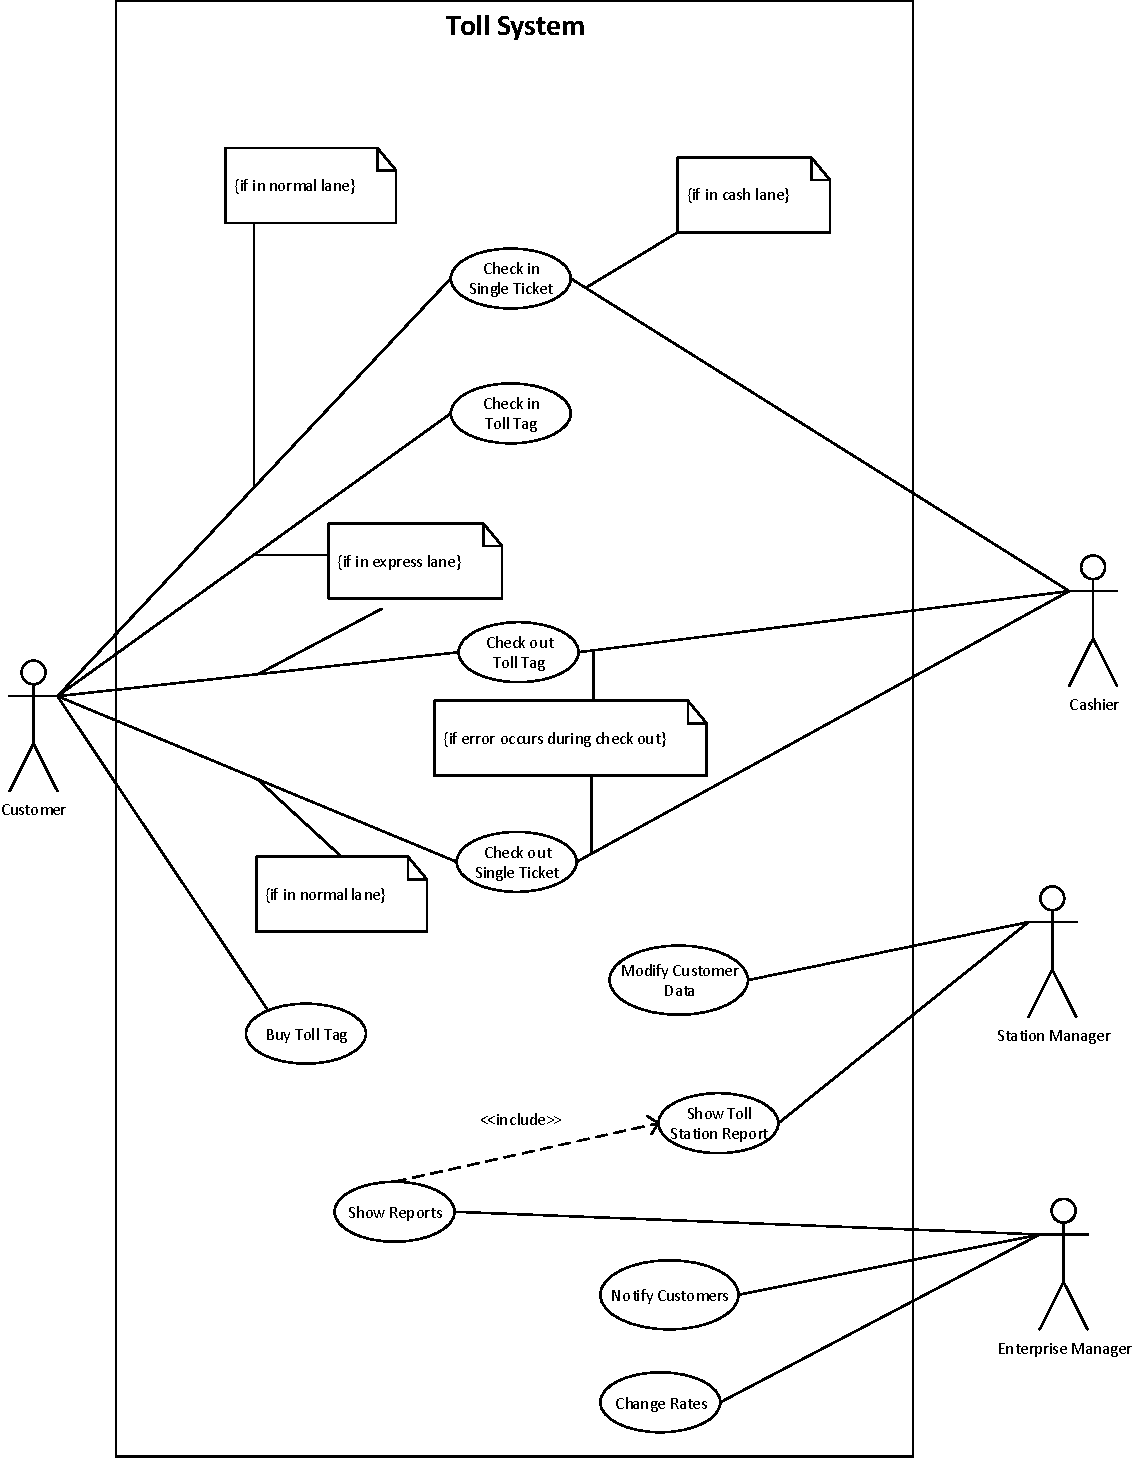
\includegraphics[width=1\textwidth]{img/use_case_diagram/use_case_diagram}
\vspace{-3cm}
\caption{The use case diagram for the toll system.}
\label{fig:use_case_diagram}
\end{figure}

The use case diagram can be seen in \autoref{fig:use_case_diagram}. It consists of the functionality of the complete system defined in the project description.

The chosen use cases are the following, as we have decided that they contain the most important functionality of the system:
\begin{enumerate}
\item Check in Single Ticket
\item Check in Toll Tag
\item Checkout Toll Tag
\item Checkout Single Ticket
\item Buy Toll Tag
\item Show Reports
\end{enumerate}

With these use cases both the single tickets and toll tags can be fully used, and statistics about the system can be generated by the enterprise manager.
